\subsection{Class Diagram}

The class diagram contains (some of) the classes used to handle three types of resources: users, rides and parks. It is possible to observe that we have a single servlet to handle the parks. Such servlet implements the doGet and doPost methods and is a subclass of the HttpServlet class. Concerning the rides, the servlet that implements the required behaviours to handle such resources is a more traditional servlet, based on the REST paradigm. In particular, we have a servlet, which also handles the Devices resource, which parses the URI, determining the type (and possibly the id) of the resource that the user wants to interact with. Once the servlet has processed the request, it forwards it to the proper Rest manager class. There are two rest manager classes: RideRestResource and DeviceRestResource. Both are sub-classes of RestResource and implement the methods to handle the proper resource. Concerning the user, there are multiple servlets used to handle the user resource. In particular, we have a servlet (UserServlet) which is mapped to URIs which are freely accessible from outside. This servlet is used to login and register new users. It has a subclass, UserServlet, which overrides the method “RegistrationOperations”, by also sending an email to the user upon registration. Note that UserServlet has been kept mainly for legacy reasons. Additionally, the UserServlet implements methods which are accessible only to users with the “admin” authorization level. In particular, it is responsible for the retrieval, update and deletion of users. Several Data Access Objects (DAOs) allow us to obtain different resources. We report the Classes that allow to handle objects of different types.
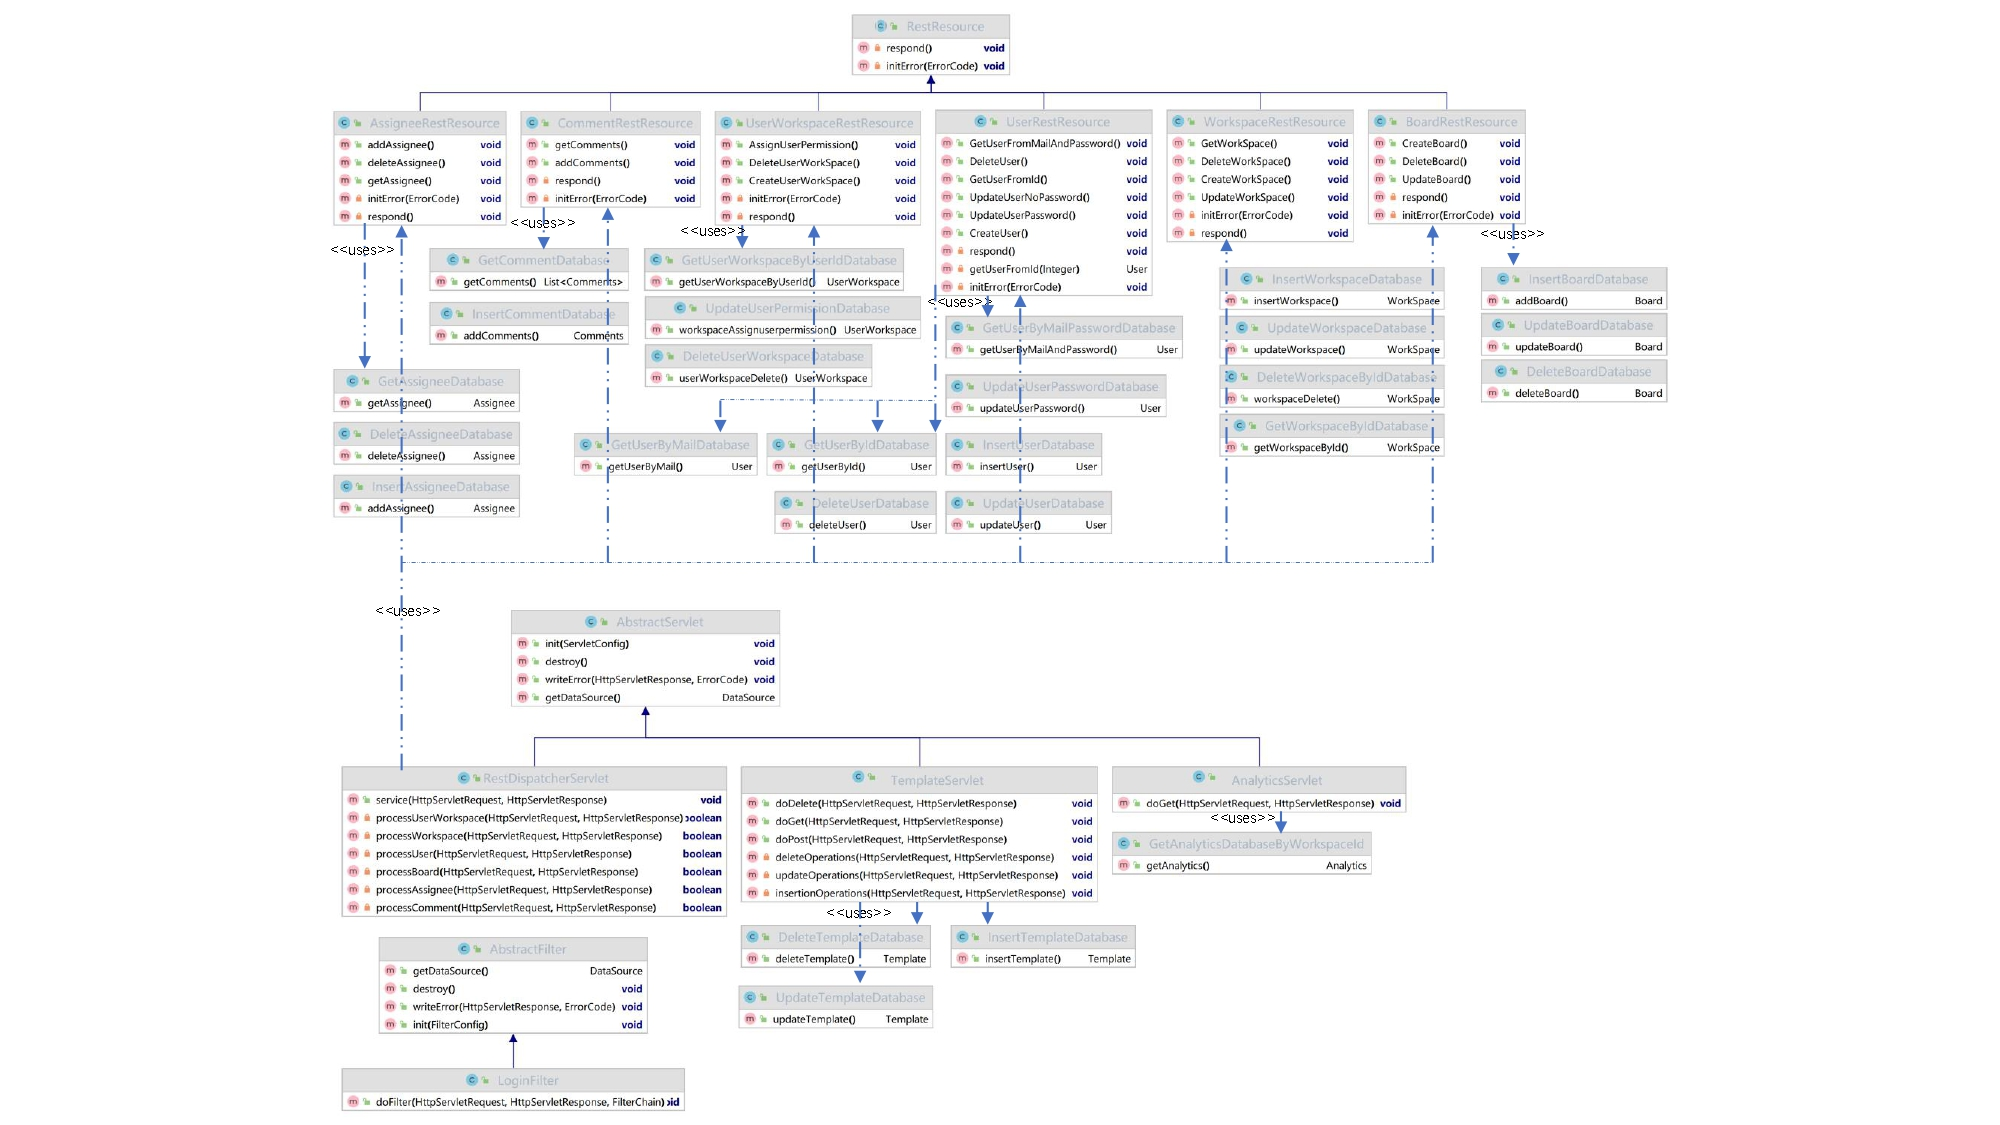
\includegraphics[width=1.30\columnwidth]{WA-workflix-HW1/images/class sequence.jpg}\\

\subsection{Sequence Diagram}
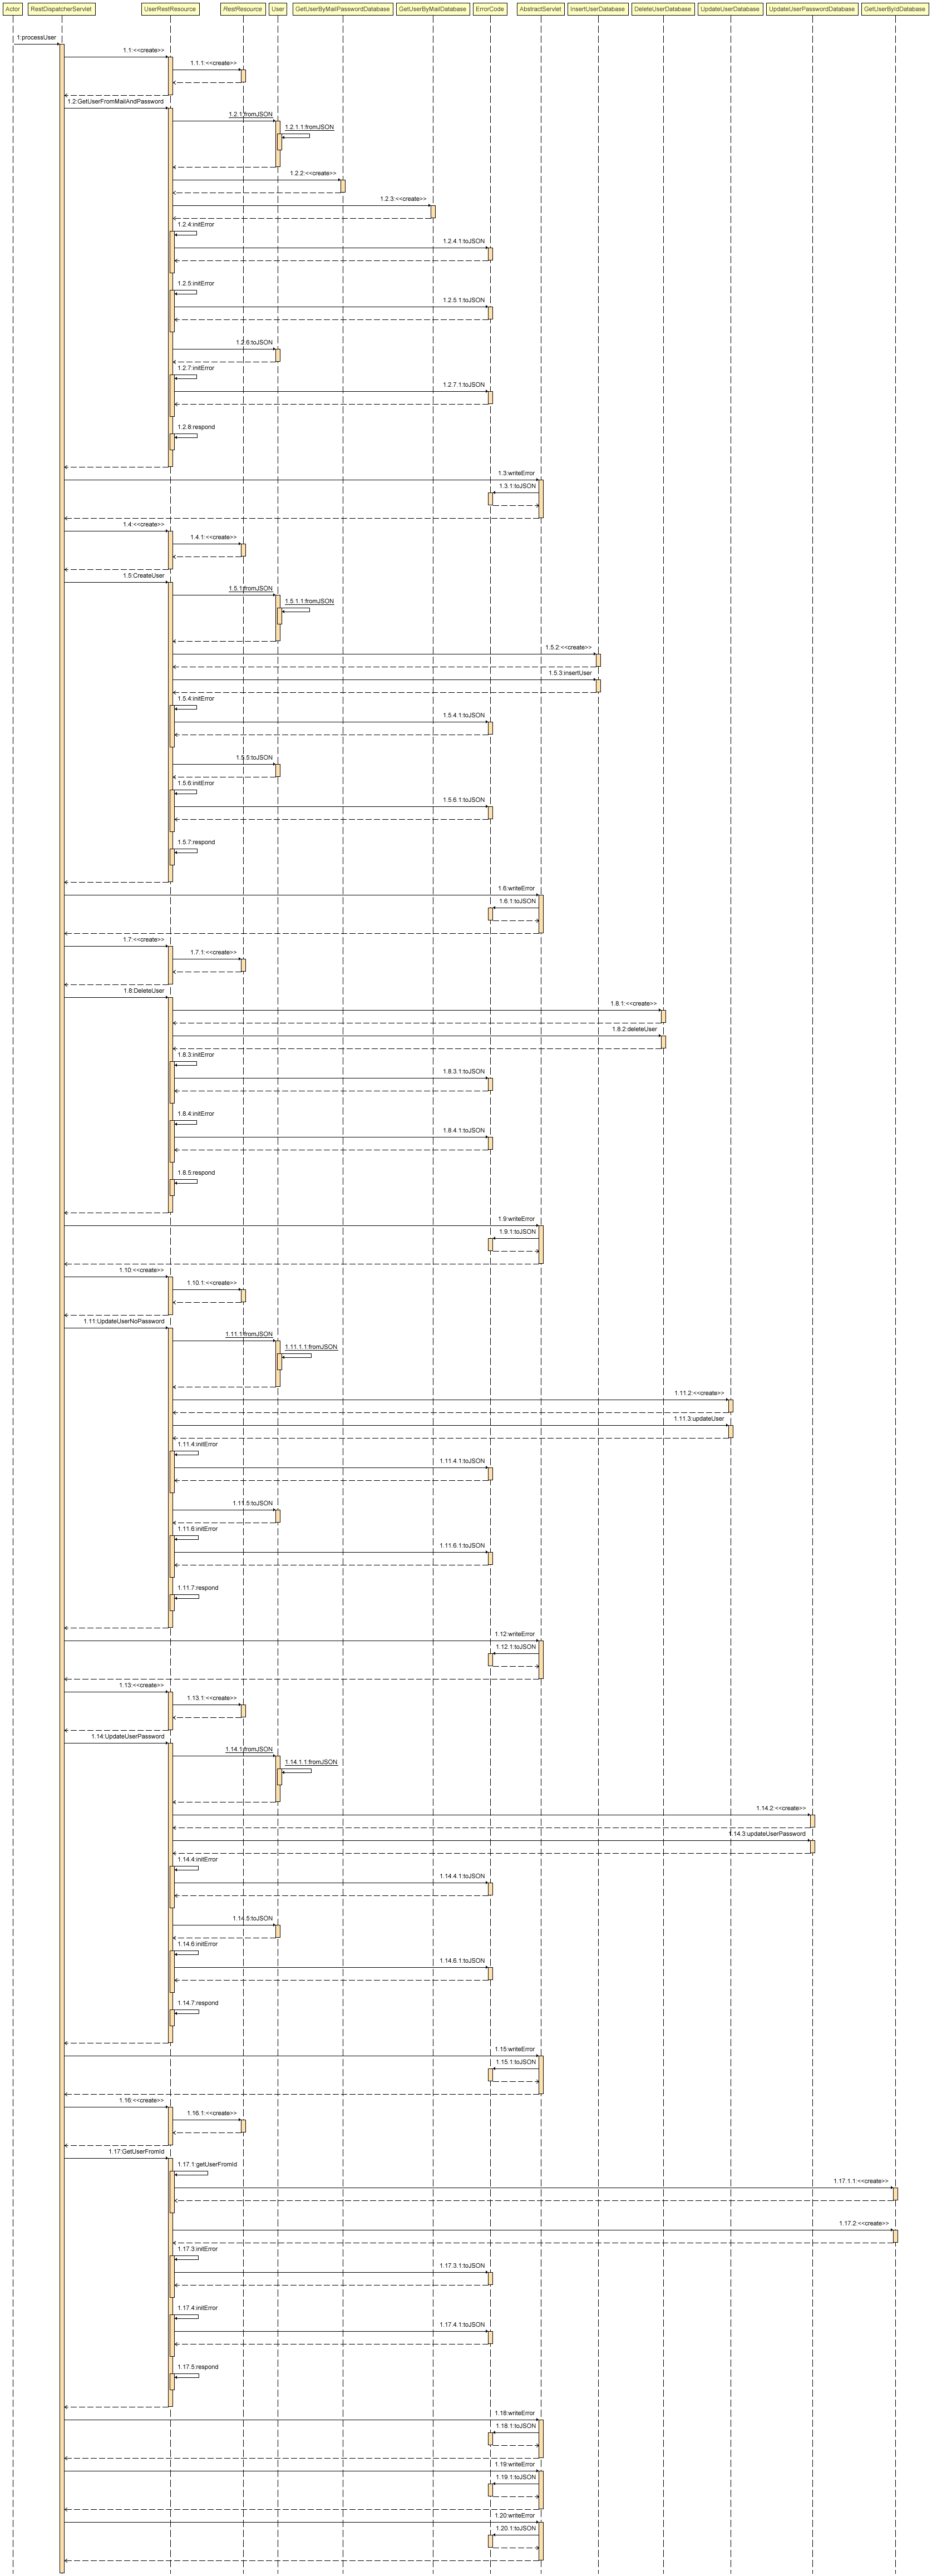
\includegraphics[width=0.5\columnwidth]{WA-workflix-HW1/images/RestDispatcherServlet_processUser.jpg}